\chapter{Organizational and People Issues}

This session from Joseph Hadzima's MIT OpenCourseWare course is not a blackboard lecture but a live panel on how ventures are built, strained, and sometimes lost through people. We should therefore preserve its rhythm: a claim is made, a practical obstacle appears, a rule of thumb is offered, and then an example complicates it. The mathematics here is correspondingly modest but still real. It lies in headcount thresholds, trial periods, scaling examples, and decision tests. These notes follow the transcript closely, and the present chapter draft is curated for book form by LazyingArt LLC.

\section{People Issues As The Dominant Failure Mode}

Hadzima opens by recalling the course's first-day framework for venture formation and then sharpens it. A successful venture requires several elements, but in practice the element most likely to fail is not technology or financing. It is the human side of the enterprise. We should read that not as a numerical theorem, but as an ordering of constraints.

\begin{equation}
\text{people issues} \succ \text{technology},
\qquad
\text{people issues} \succ \text{funding}.
\end{equation}

The panel format follows naturally from this ranking. If people issues are structurally central, then cases, counterexamples, and lived operating judgments are more revealing than a single abstract doctrine. Vivian, the moderator, frames the discussion in founder language: how we build an organization, hire, pay, solve problems, and preserve what is distinctive about the company as it grows. The other panelists then widen the lens. One speaks from large-company HR and acquisition; another from global people operations and process design. The lecture keeps moving among these scales, but its governing thesis remains fixed: people are not an accessory to the business. They are the medium through which every other part of the business either coheres or fails.

\begin{remark}
The displayed formulas in this chapter are transcript-derived heuristics rather than board equations from the room. They are included only to keep the lecture's decision logic visible.
\end{remark}

\section{Culture Starts Before HR}

The first substantial move of the panel is corrective. Culture does not begin when an HR department is hired. It begins at founding. If two or three people start a company together, then before any formal function exists they have already begun to define the organization: what quality means, what values govern the work, how they speak to one another, how trust is built, and what sort of mistakes are tolerated or corrected.

The panel repeatedly returns to four early mechanisms.

\begin{enumerate}
\item Founders must talk explicitly about what matters.
\item Trust must be assumed in part, but then built in practice.
\item Hiring behavior already creates culture, whether the founders intend it or not.
\item Routine matters: a regular cadence gives people security and makes the company legible to itself.
\end{enumerate}

This last point is unexpectedly important in the lecture. Vivian compares management to parenting in one narrow but useful sense. Predictable routines are not merely administrative; they give a team enough stability to work. If routines are absent, then every mistake feels like a crisis. If routines are present, then mistakes can become part of a usable learning process.

\subsection{Question \& Answer}

\paragraph{Question.} When should we start thinking about the HR function, and how do we preserve the company's DNA as investors arrive?

\paragraph{Answer.} The answer is earlier and later than one might expect. Earlier, because the real content of culture begins immediately, long before a formal people function exists. Later, because a tiny company does not yet need a full HR apparatus; much of the early work is still carried by founders, advisors, and careful hiring.

To make the panel's headcount logic explicit, let \(n\) denote employee headcount, and let \(\operatorname{support}(n)\) denote the amount of explicit people and organizational support the firm requires at stage \(n\). Then a fair transcript-derived compression of the discussion is

\begin{equation}
\operatorname{support}(n)=
\begin{cases}
\text{founder-led / informal}, & n<25,\\
\text{outside advice useful}, & 25\le n\le 50,\\
\text{explicit people support hard to avoid}, & n\gtrsim 50.
\end{cases}
\end{equation}

This is not a law. It is a stage heuristic. The panel is clear that the exact threshold depends on the nature of the business, but it is equally clear that by roughly the \(25\) to \(50\) range the company is usually beyond pure intuition.

\paragraph{Worked example.} The usefulness of the heuristic is not predictive precision. It is the visibility of regime change.

\begin{align}
n=12 &\Rightarrow \operatorname{support}(n)=\text{founder-led / informal},\\
n=35 &\Rightarrow \operatorname{support}(n)=\text{outside advice useful},\\
n=60 &\Rightarrow \operatorname{support}(n)=\text{explicit people support becomes urgent}.
\end{align}

At \(n=12\), alignment and daily founder attention still carry most of the organizational burden. At \(n=35\), legal, financial, and organizational advice becomes materially useful. By \(n=60\), the company can no longer assume that role design, fairness, hiring practice, and operating rhythm will take care of themselves.

\begin{figure}
\centering
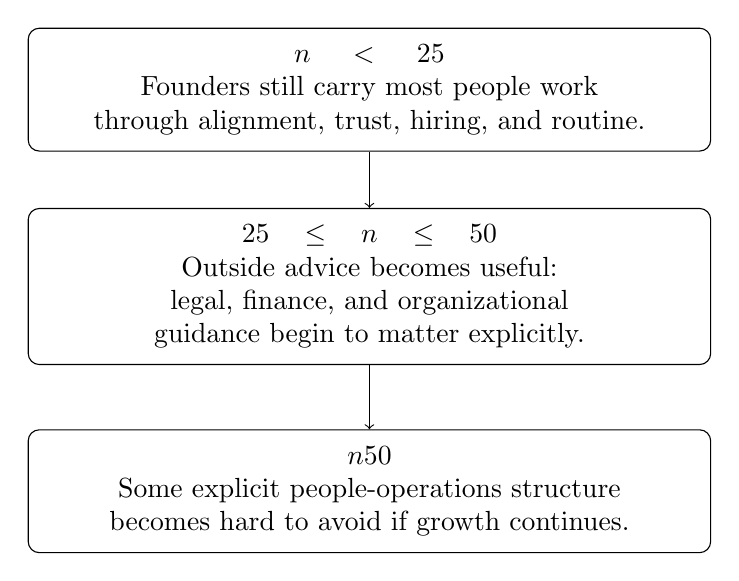
\begin{tikzpicture}
\node[draw, rounded corners, align=center, text width=0.68\linewidth, inner sep=6pt] (a) at (0,0) {$n<25$\\Founders still carry most people work\\through alignment, trust, hiring, and routine.};
\node[draw, rounded corners, align=center, text width=0.68\linewidth, inner sep=6pt] (b) at (0,-2.5) {$25\le n\le 50$\\Outside advice becomes useful:\\legal, finance, and organizational guidance begin to matter explicitly.};
\node[draw, rounded corners, align=center, text width=0.68\linewidth, inner sep=6pt] (c) at (0,-5.1) {$n\gtrsim 50$\\Some explicit people-operations structure\\becomes hard to avoid if growth continues.};
\draw[->] (a.south) -- (b.north);
\draw[->] (b.south) -- (c.north);
\end{tikzpicture}
\caption{Transcript-derived stage heuristic for people and organizational support. The boundaries are approximate, and the lecture presents them as rules of thumb rather than exact thresholds.}
\end{figure}

The lecture then adds two refinements. First, in many early companies legal or financial help arrives before HR, because payroll, taxes, and basic financial control become urgent immediately. Second, once a people function does emerge, it should not simply disappear under finance. The panel is unusually direct here: do not make HR a subordinate shadow of the finance function. The work is different and important in a different way.

Once the threshold question has been answered, the panel turns from timing to content. What exactly is the company's DNA? The answer given is mission plus recurring behavior. A mission statement matters because it allows a growing company to remind itself what all the dispersed tasks are for. The Thermo Fisher example is introduced precisely at this point: even at roughly \(130{,}000\) employees, a short mission can still locate the purpose of the work. The entrepreneurial lesson is not that one should imitate a corporate slogan, but that a company grows more coherently when employees can connect their work to a durable human purpose.

\section{Roles, Friendship, And The Co-Founder Boundary}

Once culture is on the table, the next problem appears naturally. Small teams are personal teams. Friendship, admiration, prior collaboration, and shared struggle often precede formal organization. The panel does not deny that. What it insists upon is that friendship cannot substitute for role clarity.

The lecture therefore narrows from culture in general to the structure of daily authority. If two people start a business together, then they must speak early about who does what, how disagreements are handled, what the norms of behavior are, and where final authority resides. The panel's point is not bureaucratic. It is preventive. We do not wait for these arrangements to ``evolve'' under stress. We state them before stress turns vagueness into resentment.

This is also where the lecture makes one of its clearest decision rules. Co-CEO arrangements typically do not work well. One person usually has to be in charge. That does not mean the second person is less valuable. It means the business needs a legible center of responsibility. The panel gives a concrete counterexample to false symmetry: one founder may want to be the evangelist for the product rather than the operator of the company. If that is understood early, the organization has a better chance of remaining healthy.

\subsection{Question \& Answer}

\paragraph{Question.} What is a co-founder, and when should title, control, or equity wait until fit is clearer?

\paragraph{Answer.} The panel treats the term ``co-founder'' as real but ambiguous. In the cases Vivian has seen, co-founders usually came in together. They did not arrive later and ask for the title as compensation for uncertain future value. The practical rule, then, is conservative: if the relationship is new, and the value is still being tested, do not give away title, control, or equity immediately.

This answer is not cynical. It is simply stage-aware. If someone brings truly indispensable expertise, and that expertise complements what the existing founder cannot do, then deeper commitment may make sense. But the panel repeatedly advises founders to take time, to work together on a problem, or to begin through a consultant or trial relationship. What matters is not merely that the candidate is strong. What matters is whether the candidate's strength fits the actual business and the actual team.

The lecture adds a humane refinement here. Some of the strongest working friendships are not preconditions of a company. They are outcomes of having built something demanding together. Mutual respect formed in the work is often stronger than friendship imported into the work.

\section{Hiring As A Decision Process, Not A Credential Filter}

The next pivot is from role clarity to hiring logic. Here the panel is both practical and unsentimental. Early hiring mistakes are not abstract errors. They write themselves directly into the culture of the company. Thus hiring is not just talent acquisition. It is a culture-forming decision process.

The most concrete advice in the session appears here: when in doubt, try before you buy. If a senior or high-stakes role is uncertain, bring the person in on a consulting or trial basis if the nature of the work permits it. This allows the founders to observe actual contribution, not merely self-description.

\subsection{Question \& Answer}

\paragraph{Question.} How do we test uncertain hires without locking ourselves into the wrong long-term relationship?

\paragraph{Answer.} Use a trial structure whenever the role is uncertain and the work allows it. The panel's rough timing claim is surprisingly crisp:

\begin{equation}
t_{\mathrm{fit}} \lesssim 3\text{ months} \approx 90\text{ days}.
\end{equation}

The older \(90\)-day probation period is invoked not as law but as a useful institutional analogue. One can usually tell within this horizon whether the person contributes, whether there is genuine give-and-take, and whether the relationship is likely to support the work. Sometimes, the panel adds, one can tell much sooner.

The compensation advice is similarly stage-sensitive. If possible, pay cash for a trial arrangement rather than reaching immediately for stock or a deep long-term commitment. If cash is scarce, one negotiates. But the underlying principle is the same: uncertainty should not be turned too quickly into irreversible structure.

The lecture then deepens the idea of evaluation. We are not only assessing a skill set. We are assessing a person. That is why the panel values multiple interviews and informal settings. Vivian explicitly says that she would take executive candidates to dinner and watch how they treated restaurant staff. The point is not social performance for its own sake. The point is that formal interviews can hide the human subtleties that daily work will expose very quickly.

We may summarize the hiring process recommended here as follows:

\begin{enumerate}
\item test the claimed capability;
\item observe real collaboration rather than verbal self-presentation;
\item look at the whole person, not only the technical résumé;
\item delay irreversible commitment until the fit is visible.
\end{enumerate}

In a lecture about culture, this is one of the deepest points. How we hire is one of the main ways culture is created.

\section{Growth, Acquisition, And The Structure--Bureaucracy Trade-Off}

The panel now broadens the frame. Once the first team is in place, the company must survive a market populated by larger firms, and may eventually become a target for acquisition by those same firms. The contrast between the small firm and the large firm is given in almost physical terms. Large firms have size, scale, reach, and the ability to service many needs at once. Small firms win somewhere else: speed, flexibility, closeness to the customer, and often price.

This is why the panel's competitive description is so sharp. The smaller firm can often move faster, customize more readily, and maintain stronger relationships. The large firm is slowed by rigidity. That does not mean scale is unimportant. It means scale comes with inertia, and inertia creates openings for smaller firms.

The lecture then turns acquisition from a finance story into a people story. Large firms acquire not only products but also knowledge, loyalty, and execution capacity. The panel therefore stresses retention of founders and core technical talent as part of the value being purchased. The acquired company should often be allowed to run largely intact for a while, so that the acquirer can understand what it has actually bought.

Two transcript-backed scale markers are especially useful here:

\begin{align}
n_{\mathrm{RSA}} &: 55 \rightarrow 2000,\\
t_{\mathrm{intact}} &\approx 1\text{ year}.
\end{align}

The RSA example shows that organizational needs are stage-dependent. A company that grows from roughly \(55\) people to roughly \(2{,}000\) does not remain the same organizationally, even if the values stay stable. The acquisition example makes a parallel point in time rather than headcount: one acquired unit was kept substantially intact for about a year before deeper integration.

The message is the same in both cases. Do not destroy the source of value too quickly.

\subsection{Question \& Answer}

\paragraph{Question.} When do process and hierarchy help the company, and when do they start slowing the business down?

\paragraph{Answer.} The panel is more favorable to early process than startup mythology usually is. Michelle's instinct is explicit: create SOPs out of the gate. Document what must be done. Give people a place to refer back to. The point is not permanence. Processes can change. The point is that undocumented work creates future confusion.

Vivian immediately adds the necessary correction: process is not the same thing as bureaucracy. It is possible to be structured without becoming clogged. We may make that distinction explicit by letting \(P\) denote the active process load in the company, and letting \(B(P)=1\) denote that process has crossed into bureaucracy. Then the lecture's test can be written schematically as

\begin{equation}
B(P)=1
\iff
P \text{ blocks customer needs or revenue without a compensating gain in clarity, fairness, or compliance.}
\end{equation}

This is a functional definition, not a moral one. Process is good when it makes work clearer, fairer, more compliant, and more reproducible. It becomes bureaucracy when it no longer helps the business run.

The panel gives a vivid cautionary example. Vivian joined a company at roughly \(500\) people in which basic structure still lived on spreadsheets, with no coherent job structure and no integrated system. Retrofitting that later was painful.

\begin{proposition}
If a company postpones basic structure until it is already large, the eventual repair is more expensive than early simple process.
\end{proposition}

\begin{proof}
At small scale, documentation can be introduced locally and revised incrementally. At large scale, payroll, job structure, benefits, reporting, fairness, and compliance are already coupled. Repair is then no longer local. It must be performed across the organization while the company is still operating. The transcript's \(500\)-person spreadsheet example is precisely such a late retrofit.
\end{proof}

The panel's positive model is therefore clear: simple process early, flat structures where possible, decision-making as low in the organization as one can responsibly allow, and continual testing of whether the current process still makes business sense.

\section{Founder Self-Awareness, Conflict, And Letting Go}

The next movement in the lecture is inward. A founder asks how to lead while still being herself, especially when she feels more relational than hard-edged. The panel's answer is unusually strong and worth preserving almost verbatim in spirit: do not perform a false persona. Be yourself. Become more self-aware. Then hire complements around your gaps.

This is one of the most important transitions in the session. The founders' problem is no longer merely, ``What structure should I build?'' It becomes, ``What kind of person am I inside the structure I am building?'' The panel is clear that growth does not require self-erasure. It requires accurate self-knowledge. If one founder is strategic but weak at execution, then the correct move may be to place execution-oriented people nearby rather than to spend years trying to become a different kind of person.

The lecture also answers a related question about whether people can change. The answer is yes, sometimes under profound stress or after serious life events. But that answer is immediately bounded. Founders at the beginning of a venture should not spend precious time hiring for hoped-for future transformation. Build with the person who is in front of you, not the improved person you imagine may someday emerge.

\subsection{Question \& Answer}

\paragraph{Question.} How do we surface conflict honestly, and how does a founder know when to step back rather than step in?

\paragraph{Answer.} The panel gives two linked answers.

First, conflict must be made speakable. Vivian's language is memorable: ask whether there is any ``undelivered communication.'' The theory behind this is simple and strong. If the real issue remains covert, the team cannot solve it. Once it is brought into the open, it becomes available for discussion.

\begin{equation}
\text{covert issue}
\xrightarrow{\text{named directly}}
\text{overt issue}
\xrightarrow{\text{discussion}}
\text{solvable issue}.
\end{equation}

This is why the lecture treats conflict as potentially productive rather than merely destructive. If conflict yields clarity, then clarity can improve execution.

\begin{equation}
\text{conflict} \rightarrow \text{clarity} \rightarrow \text{better execution}.
\end{equation}

Second, founders must learn when direct intervention ceases to be scaling and begins to be bottlenecking. Let \(F_{\mathrm{critical}}\) be the set of functions that must be executed reliably for the company to scale, and let \(S\) denote an informal indicator of organizational scalability. Then the lecture's late-stage warning may be written as

\begin{equation}
\Bigl(\forall f\in F_{\mathrm{critical}},\ \text{founder executes }f\Bigr)\Rightarrow S=0.
\end{equation}

\begin{proposition}
If every critical function still routes personally through the founder, the operating model is not scalable.
\end{proposition}

\begin{proof}
A single person becomes the bottleneck for judgment and action. As demand grows, delay accumulates. The founder tires, becomes irritated, begins to over-control, and the staff loses room to act. What expands is workload, not organizational capacity. The panel states this in ordinary language: doing everything yourself all the time is not a scalable model.
\end{proof}

Hadzima's own case study makes the conflict point concrete. A brilliant technical co-founder was causing slippage not by incompetence but by interactional pattern. People would bring ideas, be made to feel foolish, and then stop surfacing problems. Schedules slipped because information stopped moving. The surface failure was lateness; the deeper variable was humiliation.

\paragraph{Worked case.} The repair logic in the story is worth laying out step by step.

\begin{enumerate}
\item Observe repeated schedule slippage.
\item Ask what is not being said directly.
\item Discover that people are withholding issues because they feel belittled.
\item Name the behavior to the co-founder, and make the interaction pattern visible.
\item Experiment with a different conversational pattern until information begins to flow again.
\end{enumerate}

The lecture is realistic here. Sometimes the problem is ego and cannot easily be fixed. Sometimes it is simply lack of awareness. In both cases, what matters is that the issue be identified accurately before the team is damaged beyond repair. Radical candor, in the sense mentioned by the panel, is not cruelty. It is honest speech delivered in a usable way.

\section{Culture As A Selection Rule And A CEO Obligation}

The closing movement of the lecture loops back through several late questions: delegated hiring, insecurity inside the hiring team, AI tools, self-awareness methods, the trade-off between brilliance and disruption, the timing of HR, and the CEO's role in preserving culture across scale and geography. What ties these apparently separate questions together is simple: the company now has to scale judgment without losing the human quality that made the early organization effective.

The hiring discussion returns in a more refined form. Once managers are hiring beneath the founder, the founder must stay close enough to the process to see whether insecurity is distorting it. The hiring manager should usually make the final decision, but the process must still have clear decision rights. Group input is useful; group indecision is expensive. The panel has seen inclusive hiring processes become so elaborate that candidates were lost.

The panel's AI remarks belong to the lecture's moment and should be read that way. Tools such as ChatGPT or LinkedIn-assisted platforms can reduce the cost of documentation, search, and drafting. They do not replace judgment in leadership, hiring, or human diagnosis. The same is true of self-awareness tools such as the Process Communication Model mentioned late in the session. They may help a team think more clearly about stress responses and communication styles, but they are aids to reflection, not substitutes for it.

\subsection{Question \& Answer}

\paragraph{Question.} Should we hire the brilliant but culturally risky person, and what kind of culture can actually scale?

\paragraph{Answer.} The panel refuses a simplistic answer. Technical brilliance matters. But the lecture insists on distinguishing between eccentricity and toxicity. Some technically extraordinary people are difficult but manageable. Others carry core character flaws that will poison a small team.

If we let \(T\) denote technical contribution and \(R\) denote cultural or behavioral risk, then the lecture's late hiring rule may be compressed into the following decision surface:

\begin{equation}
D(T,R)=
\begin{cases}
\text{hire}, & T\text{ high},\ R\text{ low},\\
\text{manage carefully}, & T\text{ high},\ R\text{ moderate and containable},\\
\text{do not hire}, & R\text{ signals toxic character}.
\end{cases}
\end{equation}

The middle case is important. The panel gives one concrete justification for it: a technically extraordinary person may advance the company's technology enough to be worth careful management, or may be worth keeping away from competitors. But even here the language is conditional. If the issue is mean-spiritedness, narcissism, or another deep character defect, then the hire is too dangerous. A small firm cannot afford that toxicity.

The broader cultural answer is equally strong. Culture scales when it is written, repeated, and embodied by the CEO. The lecture gives several versions of this claim. One is the simple mission statement. Another is the ``people first'' founder who believed that if the company took care of its people, the people would take care of the customers. Another is the CEO who travels, remains close to employees, and does not disappear into hierarchy. The RSA example is used to show that a strong culture can remain recognizable across roughly twenty countries even while each local office keeps local variation.

What cannot scale is pure founder centrality. What can scale is a mission people can remember, decision rights people can understand, and a style of treatment people can trust. The final lesson is subtle but decisive. Culture is not what the company says about itself once a year. It is what people learn from the company's recurring acts: whom it hires, what it tolerates, how it corrects, whom it trusts, and how its leaders behave when the stakes are high.

\section{Summary}

This lecture contains almost no formal mathematics in the usual sense, but it does contain a precise operational logic. We move from an ordering of failure modes, to headcount thresholds, to trial periods, to structure tests, to scalability constraints. Along the way the panel keeps refusing two false alternatives: culture versus performance, and structure versus agility. The best organizations in the lecture are not soft. They are demanding and humane at the same time.

The chapter's central claim is therefore the same as the lecture's opening claim, now made more explicit. A venture does not merely have people issues among its other issues. People are the mechanism through which all the other issues are managed. That is why the session begins with failure, passes through hiring and role clarity, turns to process and acquisition, and ends with self-awareness, trust, and CEO behavior. The company grows only insofar as its human system grows with it.